\documentclass{article}

% Language setting
% Replace `english' with e.g. `spanish' to change the document language
\usepackage[english]{babel}

% Set page size and margins
% Replace `letterpaper' with `a4paper' for UK/EU standard size
\usepackage[letterpaper,top=2cm,bottom=2cm,left=3cm,right=3cm,marginparwidth=1.75cm]{geometry}

% Useful packages
\usepackage{amsmath}
\usepackage{graphicx}
\usepackage[colorlinks=true, allcolors=blue]{hyperref}

\title{FEA slow control}
\author{Romain Ga\"ior}

\begin{document}
\maketitle

\begin{abstract}
Description and operation of the slow control system used for the Field Array Emission setup at IPMU Kamioka branch. 
\end{abstract}

\section{Introduction}
\begin{figure}
\centering
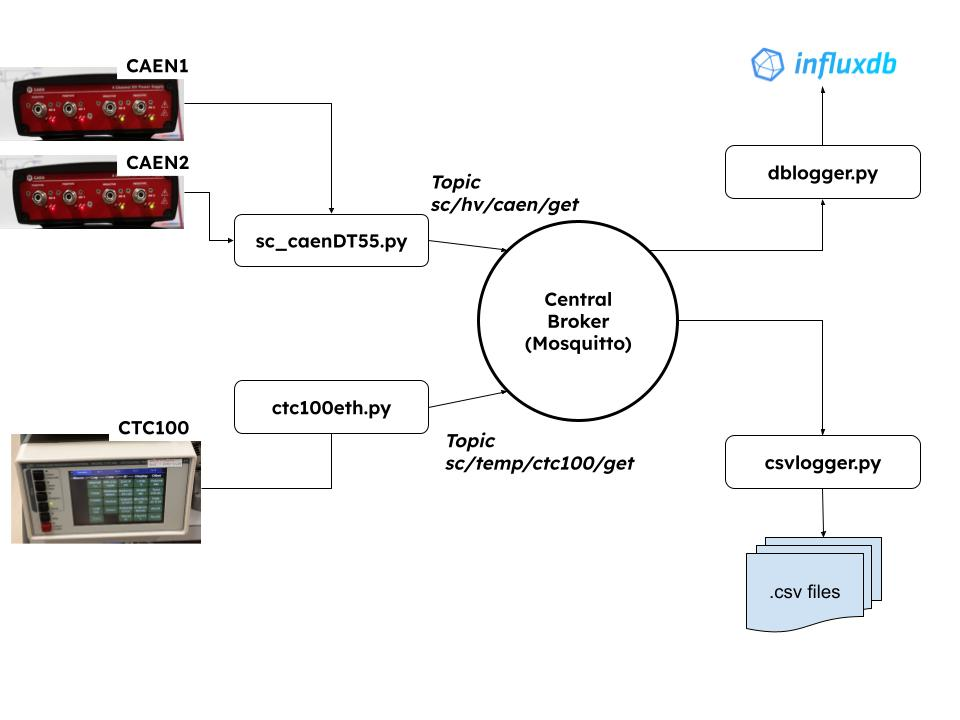
\includegraphics[width=0.9\linewidth]{fea_sc.jpg}
\caption{\label{fig:sc}general sketch of the slow control system}
\end{figure}

The system controls:
\begin{itemize}
    \item two CAEN HV power supplies 
    \item one cryogenic controller
\end{itemize}
\subsection{Description}
It's implemented using a communication protocol called MQTT [\url{https://mqtt.org/}]. MQTT is a protocol based on message publishing and subscribing and a central broker which distribute the message from the publisher to the relevant subscribers. The control of the two instruments works the same way: one python script query the data on the ethernet link from the PC to the device and publishes the result on a given topic. Then there are other scripts which are subscriber of the topic and that either log the data in the data base or write them in a file or just display the message. See the sketch in Fig.\ref{fig:sc}.\\
The code is available on github: \url{https://github.com/rgaior/fea_sc.git}.

\subsection{Installation}
\paragraph{PC}
\begin{itemize}
    \item distribution: LMDE 6 (faye)
    \item CPU intel I7 64 bit, RAM 8GB
    \item username: xenon
    \item IP: \verb|10.240.102.252|  
\end{itemize}

\paragraph{Device addresses}
\begin{itemize}
    \item CAEN1 (PID 58374): \verb|192.168.0.250|
    \item CAEN2: (PID14133): \verb|192.168.0.251|
    \item CTC100: \verb|192.168.0.252|
\end{itemize}

\paragraph{influxdb}
\begin{itemize}
    \item local installation
    \item \begin{verbatim} InfluxDB v2.7.6 (git: 3c58c06206) build_date: 2024-04-12T21:51:21Z \end{verbatim}
    \item account : username = ipmu ; pw = same as the computer
    \item UI: http://10.240.102.252:8086/
    \item bucket:\verb | FEA_SC |
    \item org: IPMU
    \item token: \begin{verbatim}u0aOHcX1oQHJUg69ucy9iWnStCeNBuuC_S-3BMtKkWH7B9pjWhf-nw3hgvpnVHuvekZqWO_I_-eNlZGWR7ggyg==\end{verbatim}
\end{itemize}

\paragraph{code location and environment}
The main repository is \verb|/home/xenon/slowcontrol/|, it contains the data (\verb |/datalogs/| ), the logs (\verb |/logs/|), the environment(\verb |/sc_venv/|)  and the code (\verb |/fea_sc/|). 

In order to activate the environment, type: \begin{verbatim}
    source /home/xenon/slowcontrol/sc_venv/bin/activate
\end{verbatim}

\section{Operation}
\subsection{Logging}
The code are python script that are run in interactive mode, so if you want to run only the data query of the  ctc100 for instance you should type:
\begin{verbatim}
    python -i ctc100/ctc100eth.py
\end{verbatim}
The CAEN HV take the argument (caen1 or caen2) to run:
\begin{verbatim}
    python -i caendt55/sc_caendt55.py caen1
\end{verbatim}
This will run a python shell and start querying the data from the device in a separate thread.
Similarly if you want to log the data you need to run the dedicated codes:
\begin{verbatim}
  python -i datalogger/csvlogger.py 
  python -i datalogger/dblogger.pypython 
\end{verbatim}

\subsection{CAEN Control}
For the control of the CAEN, in the python shell opened with \verb|sc_caendt55.py| code,  one can simply type 
\begin{verbatim}
    caenhv.set(channel, PARAM, value)
\end{verbatim}
where channel is 0,1,2,3 PARAM are listed in the CAEN power supply manual (see the screen shot in Fig.~\ref{fig:setcommands}) and value is the value you want to set.

\subsection{CAEN display}
In the case of the CAEN we want to log, control and display the output values. These operations are done with separate scripts (\verb|sc_caendt55.py| for the control and \verb|caen_display.py| for the display). The display is run with 
\begin{verbatim}
    python -i caendt55/caen_display.py caen1
\end{verbatim}
This will open a python shell with the information of the CAEN displayed  
\begin{figure}
\centering
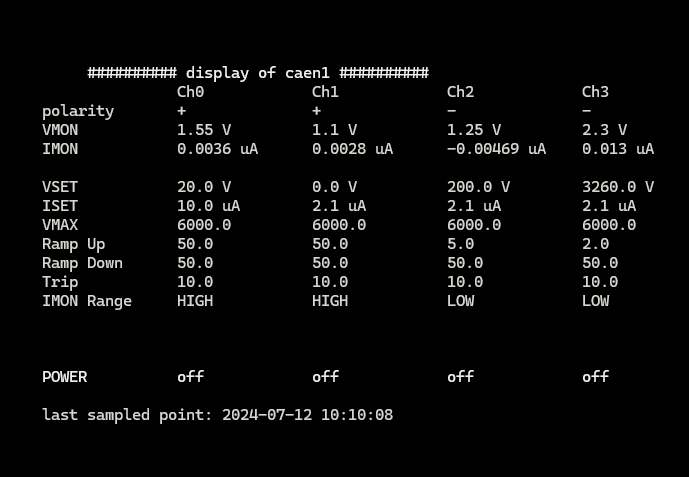
\includegraphics[width=0.45\linewidth]{caen_display.png}
    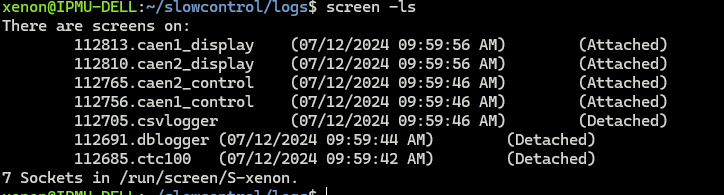
\includegraphics[width=0.45\linewidth]{image.png}
\caption{\label{fig:caen_display}display of the CAEN HV information}
\end{figure}

\subsection{Scripts}
There are some bash script to open automatically the monitoring parts in different \verb|screen| sessions:
\begin{itemize}
    \item \verb|/slowcontrol/start_ctc.sh| : start the ctc logging    
    \item \verb|/slowcontrol/start_caen.sh|: start the CAEN logging, control and display and puts that in a TMUX window Fig.~\ref{fig:caen_all}
    \item \verb|/slowcontrol/start_logger.sh| : start the code to push data in db and in csv file.
    \item \verb|/slowcontrol/start_sc.sh| : start the above scripts
\end{itemize}
At the end, when all the script are executed one should see a list of screens like in Fig.~\ref{fig:caen_display} (right).


The CAEN control and display window are in a TMUX so you need to know the related commands.
\begin{itemize}
    \item to detach from the TMUX window: \verb|ctrl-b d| 
    \item to list the TMUX session: \verb|tmux ls|
    \item to attach from the TMUX window: \verb|tmux attach -t <name of the session>| or \verb|tmux a| if there is only one session.  
    \item To navigate between the panes with \verb|ctrl-b| $\leftarrow \rightarrow \uparrow \downarrow$
\end{itemize}
So you can set a value in the CAEN control part and see the result instantaneously in the CAEN display part. 

\begin{figure}
\centering
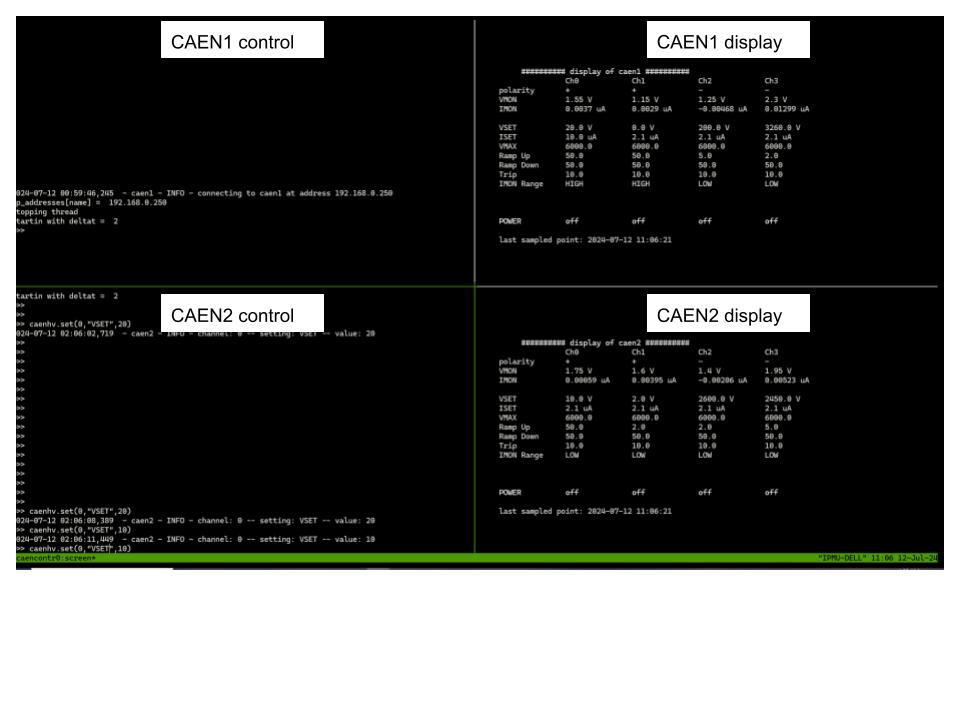
\includegraphics[width=0.9\linewidth]{caen_all.jpg}
\caption{\label{fig:caen_all}CAEN TMUX window for control and display}
\end{figure}
\subsection{logs}
\begin{itemize}
    \item The logs of action are recorded in the folder: \verb|/slowcontrol/logs/|
    \item The csv file are store in the folder: \verb|/slowcontrol/datalogs/| 
\end{itemize}

\appendix
\section{set commands}

\begin{figure}
\centering
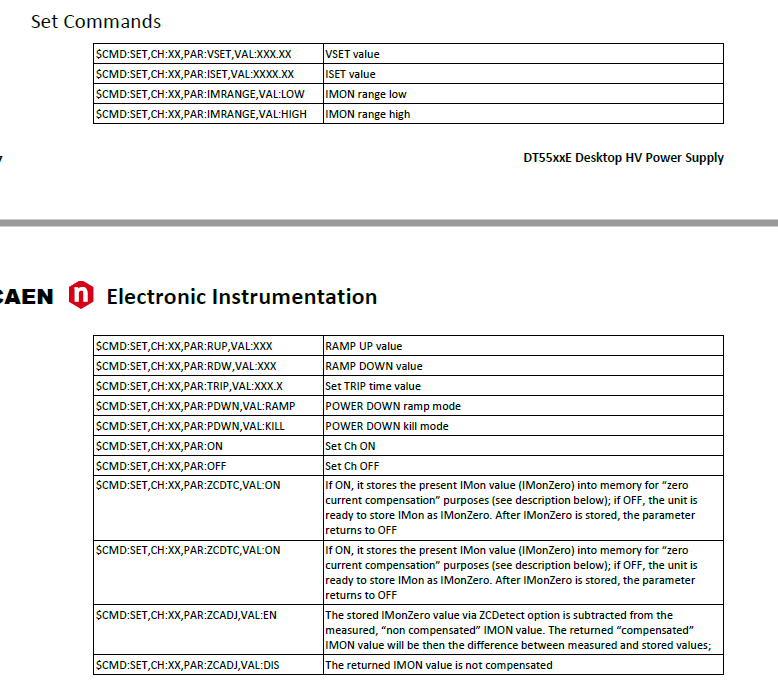
\includegraphics[width=0.9\linewidth]{setcommands.png}
\caption{\label{fig:setcommands}}
\end{figure}



%\bibliographystyle{alpha}
%\bibliography{sample}

\end{document}